\chapter{PENGUJIAN DAN EVALUASI}
\par Bab ini membahas pengujian dan evaluasi terhadap perangkat lunak yang telah diimplementasikan dengan menggunakan metode \textit{blackbox}.

\section{Lingkungan Pengujian}
\par Lingkungan yang digunakan untuk menguji tugas akhir ini memiliki spesifikasi perangkat keras dan lunak yang ditunjukkan pada Tabel \ref{t:spec-server}, \ref{t:spec-android}, \ref{t:spec-android-2}, \ref{t:spec-android-3}, dan \ref{t:spec-ios}. Implementasi aplikasi android yang digunakan untuk pengujian dapat dilihat pada \nameref{lampiran:implementasi-android}.
\begin{longtable}{|p{3cm}|p{6cm}|}
	\caption{Spesifikasi Server} \label{t:spec-server} \\ \hline
    \rowcolor{lightgray} Komponen & Spesifikasi \\ \hline
    \endfirsthead
    \hline
    \rowcolor{lightgray} Komponen & Spesifikasi \\ \hline
    \endhead
    CPU & Intel(R) Xeon(R) CPU E5-2690 v4 \\ \hline
    CPU Core & 4 \\ \hline
    Memory & 8 GB \\ \hline
    Sistem Operasi & Ubuntu 18.04 \\ \hline
\end{longtable}
\begin{longtable}{|p{3cm}|p{6cm}|}
	\caption{Spesifikasi Perangkat Android 1} \label{t:spec-android} \\ \hline
	\rowcolor{lightgray} Komponen & Spesifikasi \\ \hline
	\endfirsthead
	\hline
	\rowcolor{lightgray} Komponen & Spesifikasi \\ \hline
	\endhead
    CPU & Snapdragon 636 \\ \hline
    Memory & 3 GB \\ \hline
    Sistem Operasi & Android 9 (Pie) \\ \hline
    Aplikasi & Push Notification Dev versi 1.0 \\ \hline
\end{longtable}
\begin{longtable}{|p{3cm}|p{6cm}|}
	\caption{Spesifikasi Perangkat Android 2} \label{t:spec-android-2} \\ \hline
	\rowcolor{lightgray} Komponen & Spesifikasi \\ \hline
	\endfirsthead
	\hline
	\rowcolor{lightgray} Komponen & Spesifikasi \\ \hline
	\endhead
	CPU & Snapdragon 625 \\ \hline
	Memory & 4 GB \\ \hline
	Sistem Operasi & Android 7 (Nougat) \\ \hline
	Aplikasi & Push Notification Dev versi 1.0 \\ \hline
\end{longtable}
\begin{longtable}{|p{3cm}|p{6cm}|}
	\caption{Spesifikasi Perangkat Android 3} \label{t:spec-android-3} \\ \hline
	\rowcolor{lightgray} Komponen & Spesifikasi \\ \hline
    \endfirsthead
    \hline
    \rowcolor{lightgray} Komponen & Spesifikasi \\ \hline
    \endhead
    CPU & Snapdragon 616 \\ \hline
    Memory & 3 GB \\ \hline
    Sistem Operasi & Android 5.1.1 (Lollipop) \\ \hline
    Aplikasi & Push Notification Dev versi 1.0 \\ \hline
\end{longtable}
\begin{longtable}{|p{3cm}|p{6cm}|}
	\caption{Spesifikasi Perangkat iOS} \label{t:spec-ios} \\ \hline
	\rowcolor{lightgray} Komponen & Spesifikasi \\ \hline
	\endfirsthead
	\hline
	\rowcolor{lightgray} Komponen & Spesifikasi \\ \hline
	\endhead
    CPU & Apple A10 Fusion \\ \hline
    Memory & 3 GB \\ \hline
    Sistem Operasi & iOS 12 \\ \hline
    Aplikasi & MyITS Wali versi 1.0.2 \\ \hline
\end{longtable}

\section{Pengujian Fungsional}
\par Pengujian fungsional dilakukan untuk mengetahui apakah sistem yang dibangun sudah memiliki kebutuhan fungsional yang diperlukan.

\subsection{Pengujian Pembuatan Packet}
\par Pengujian pembuatan \textit{packet} dilakukan untuk mengetahui apakah Scheduler berhasil membuatkan data \textit{packet} dari \textit{batch} dengan tepat. Hasil uji dapat dilihat pada Tabel \ref{t:uji_pembuatan_packet}.
\begin{longtable}{|>{\columncolor{lightgray}}p{3cm}|p{6.5cm}|}
	\caption{Hasil Uji Pembuatan \textit{Packet}} \label{t:uji_pembuatan_packet} \\ \hline
	\endfirsthead
	Kode & FT-01 \\ \hline
	Nama & Pengujian Pembuatan \textit{Packet} \\ \hline
	Tujuan & Menguji apakah sistem mampu membuatkan data \textit{packet} dari data \textit{batch} \\ \hline
	Kondisi Awal & Scheduler aktif \\ \hline
	Langkah Pengujian &  
	\begin{enumerate}
		\item Pengguna menambahkan data \textit{batch} baru lewat halaman kirim notifikasi di modul manajemen.
		\item Setelah 30 detik, data \textit{packet} akan disimpan di sistem basis data.
	\end{enumerate} \\ \hline
	Hasil yang diharapkan & Data \textit{packet} tersimpan di sistem basis data \\ \hline
	Hasil yang diperoleh & Data \textit{packet} tersimpan di sistem basis data \\ \hline
	Hasil pengujian & Berhasil \\ \hline
\end{longtable}

\subsection{Pengujian Menambahkan Packet ke Antrian}
\par Pengujian menambahkan \textit{packet} dilakukan untuk mengetahui apakah Scheduler berhasil menambahkan \textit{packet} ke antrian dengan tepat. Hasil uji dapat dilihat pada Tabel \ref{t:uji_pembuatan_antrian}.
\begin{longtable}{|>{\columncolor{lightgray}}p{3cm}|p{6.5cm}|}
	\caption{Hasil Uji Menambahkan \textit{Packet} ke Antrian} \label{t:uji_pembuatan_antrian} \\ \hline
	\endfirsthead
	Kode & FT-02 \\ \hline
	Nama & Pengujian Pembuatan Antrian \\ \hline
	Tujuan & Menguji apakah sistem mampu membuatkan data antrian dari data \textit{packet} \\ \hline
	Kondisi Awal & Scheduler aktif \\ \hline
	Langkah Pengujian &  
	\begin{enumerate}
		\item Pengguna menambahkan data \textit{batch} baru lewat halaman kirim notifikasi di modul manajemen.
		\item 30 detik setelah waktu pengiriman \textit{batch}, data \textit{packet} untuk \textit{batch} akan tersimpan di sistem antrian pesan.
	\end{enumerate} \\ \hline
	Hasil yang diharapkan & Data \textit{packet} tersimpan di sistem antrian pesan. \\ \hline
	Hasil yang diperoleh & Data \textit{packet} tersimpan di sistem antrian pesan. \\ \hline
	Hasil pengujian & Berhasil \\ \hline
\end{longtable}

\subsection{Pengujian Pengiriman Packet ke APNs}
\par Pengujian pengiriman \textit{packet} ke APNs dilakukan untuk mengetahui apakah Sender APN berhasil mengirimkan \textit{packet} ke layanan APNs dengan tepat. Hasil uji dan notifikasi dapat dilihat pada Tabel \ref{t:uji_pengiriman_packet_apn} dan Gambar \ref{f:ss_ios}.
\begin{longtable}{|>{\columncolor{lightgray}}p{3cm}|p{6.5cm}|}
	\caption{Hasil Uji Pengiriman \textit{Packet} ke APNs} \label{t:uji_pengiriman_packet_apn} \\
	\endfirsthead \hline
	Kode & FT-03 \\ \hline
	Nama & Pengujian Pembuatan \textit{Packet} \\ \hline
	Tujuan & Menguji apakah sistem mampu mengirim \textit{packet} lewat layanan APNs \\ \hline
	Kondisi Awal & Scheduler dan Sender APN aktif \\ \hline
	Langkah Pengujian &  
	\begin{enumerate}
		\item Pengguna menambahkan data \textit{batch} baru untuk perangkat iOS lewat halaman kirim notifikasi di modul Manajemen.
		\item 1 menit setelah waktu pengiriman \textit{batch}, notifikasi akan diterima oleh perangkat iOS.
	\end{enumerate} \\ \hline
	Hasil yang diharapkan & Notifikasi diterima oleh perangkat iOS \\ \hline
	Hasil yang diperoleh & Notifikasi diterima oleh perangkat iOS \\ \hline
	Hasil pengujian & Berhasil \\ \hline
\end{longtable}
\begin{figure}[H]
	\centering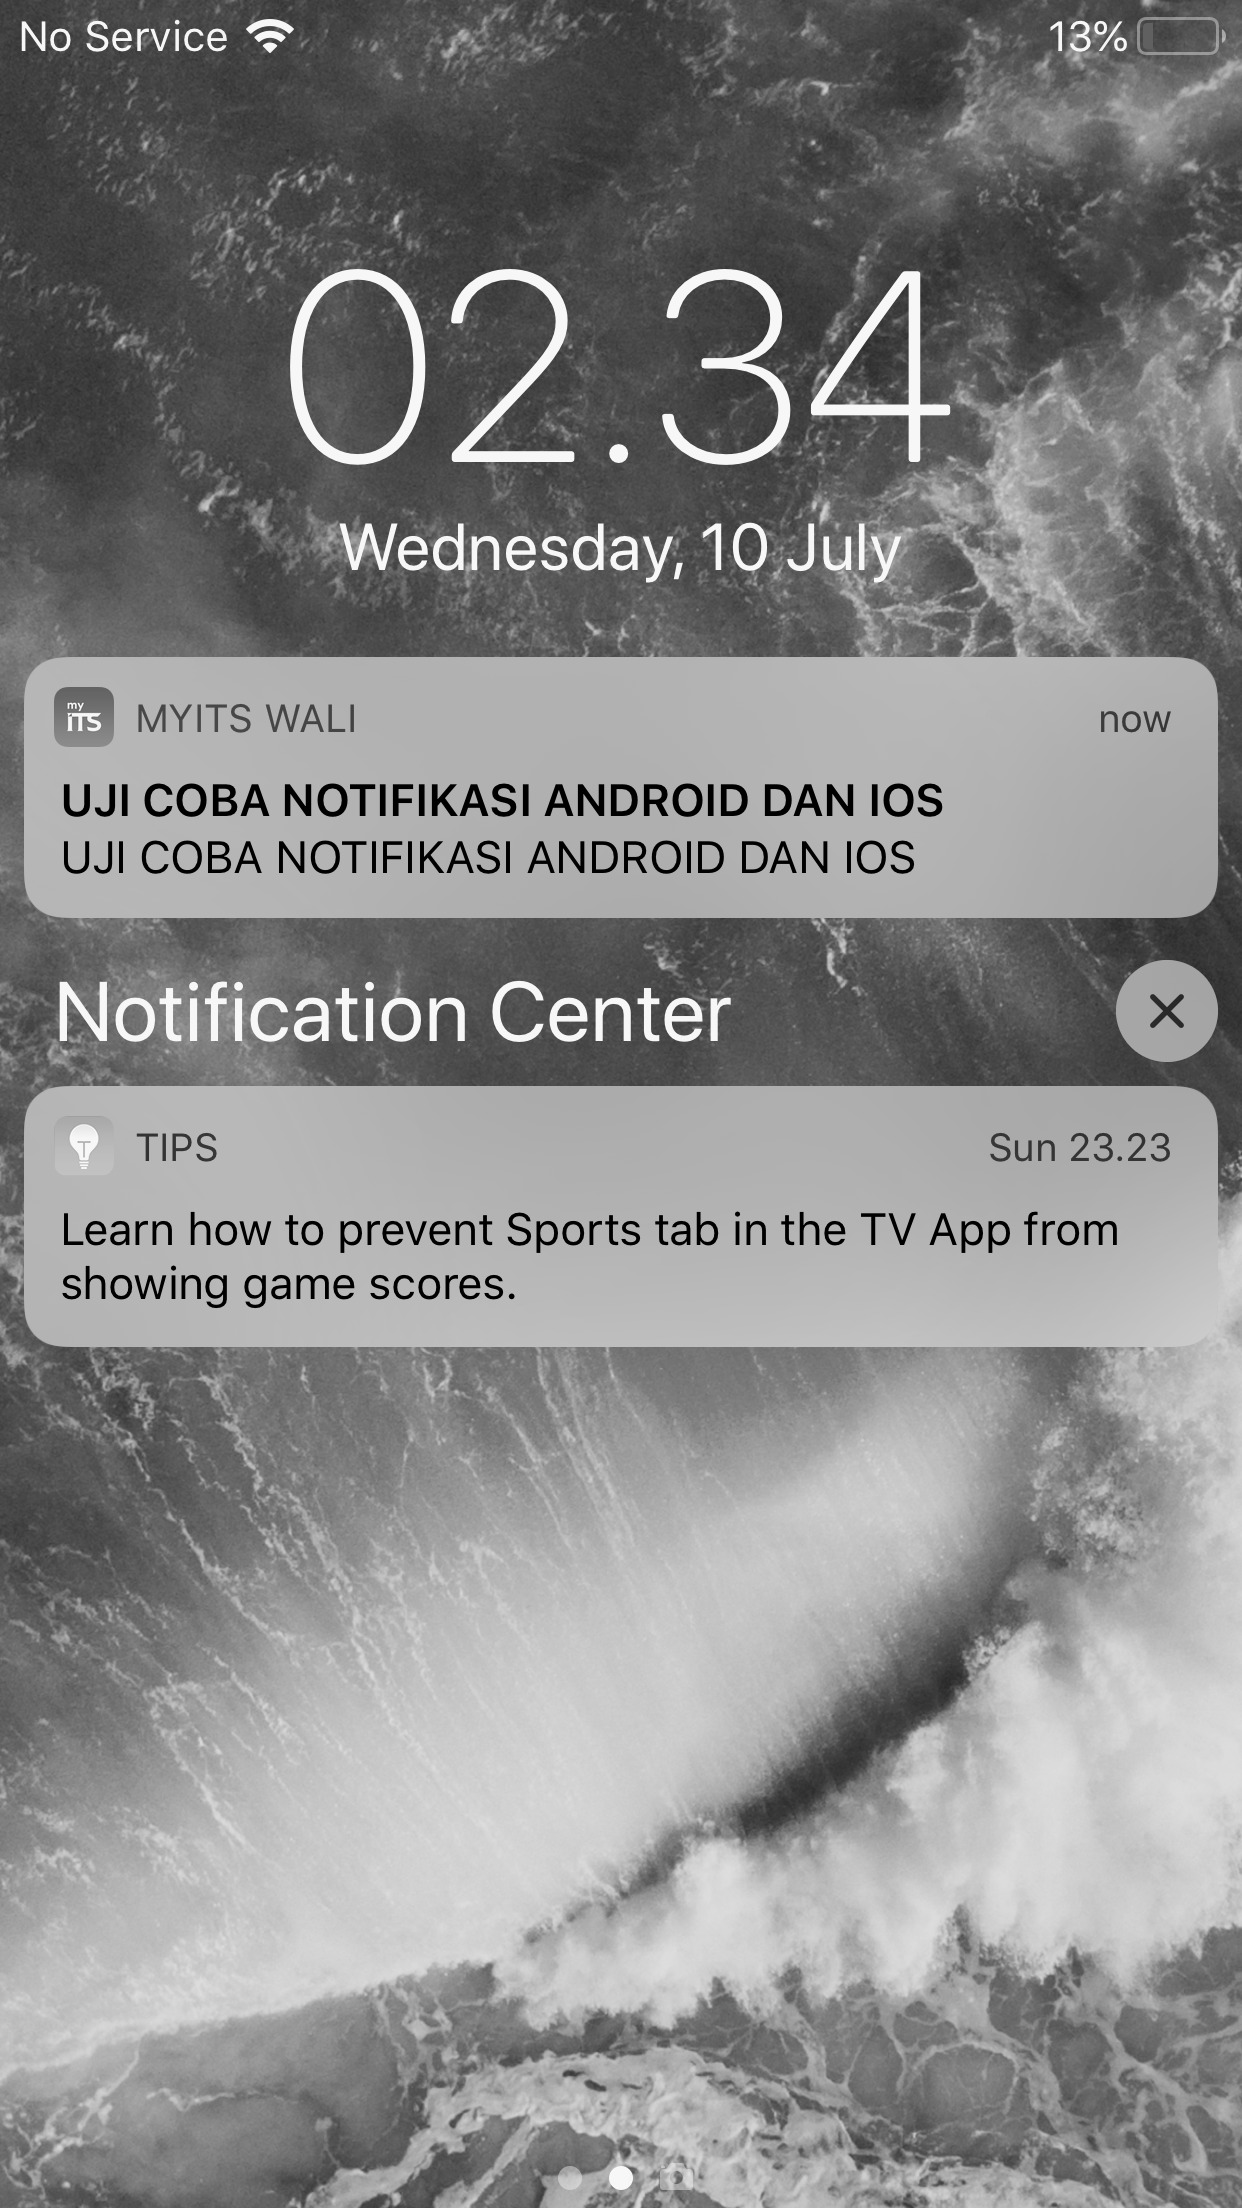
\includegraphics[width=0.35\textwidth]{bab5/img/notifikasi-ios.jpg}
	\caption{Hasil Notifikasi pada Perangkat iOS} \label{f:ss_ios}
\end{figure}

\subsection{Pengujian Pengiriman Packet ke FCM}
\par Pengujian pengiriman \textit{packet} ke FCM dilakukan untuk mengetahui apakah Sender FCM berhasil mengirimkan \textit{packet} ke layanan FCM dengan tepat. Hasil uji dan notifikasi dapat dilihat pada Tabel \ref{t:uji_pengiriman_packet_fcm} dan Gambar \ref{img:notifikasi-android}.
\begin{longtable}{|>{\columncolor{lightgray}}p{3cm}|p{6.5cm}|}
	\caption{Hasil Uji Pengiriman \textit{Packet} ke FCM} \label{t:uji_pengiriman_packet_fcm} \\ \hline
	\endfirsthead
	Kode & FT-04 \\ \hline
	Nama & Pengujian Pengiriman \textit{Packet} ke FCM \\ \hline
	Tujuan & Menguji apakah sistem mampu mengirim \textit{packet} lewat layanan FCM \\ \hline
	Kondisi Awal & Scheduler dan Sender FCM aktif \\ \hline
	Langkah Pengujian &  
	\begin{enumerate}
		\item Pengguna menambahkan data \textit{batch} baru untuk perangkat Android lewat halaman kirim notifikasi di modul Manajemen.
		\item 1 menit setelah waktu pengiriman \textit{batch}, notifikasi akan diterima oleh perangkat Android.
	\end{enumerate} \\ \hline
	Hasil yang diharapkan & Notifikasi diterima oleh perangkat Android \\ \hline
	Hasil yang diperoleh & Notifikasi diterima oleh perangkat Android \\ \hline
	Hasil pengujian & Berhasil \\ \hline
\end{longtable}
\begin{figure}[H]
	\centering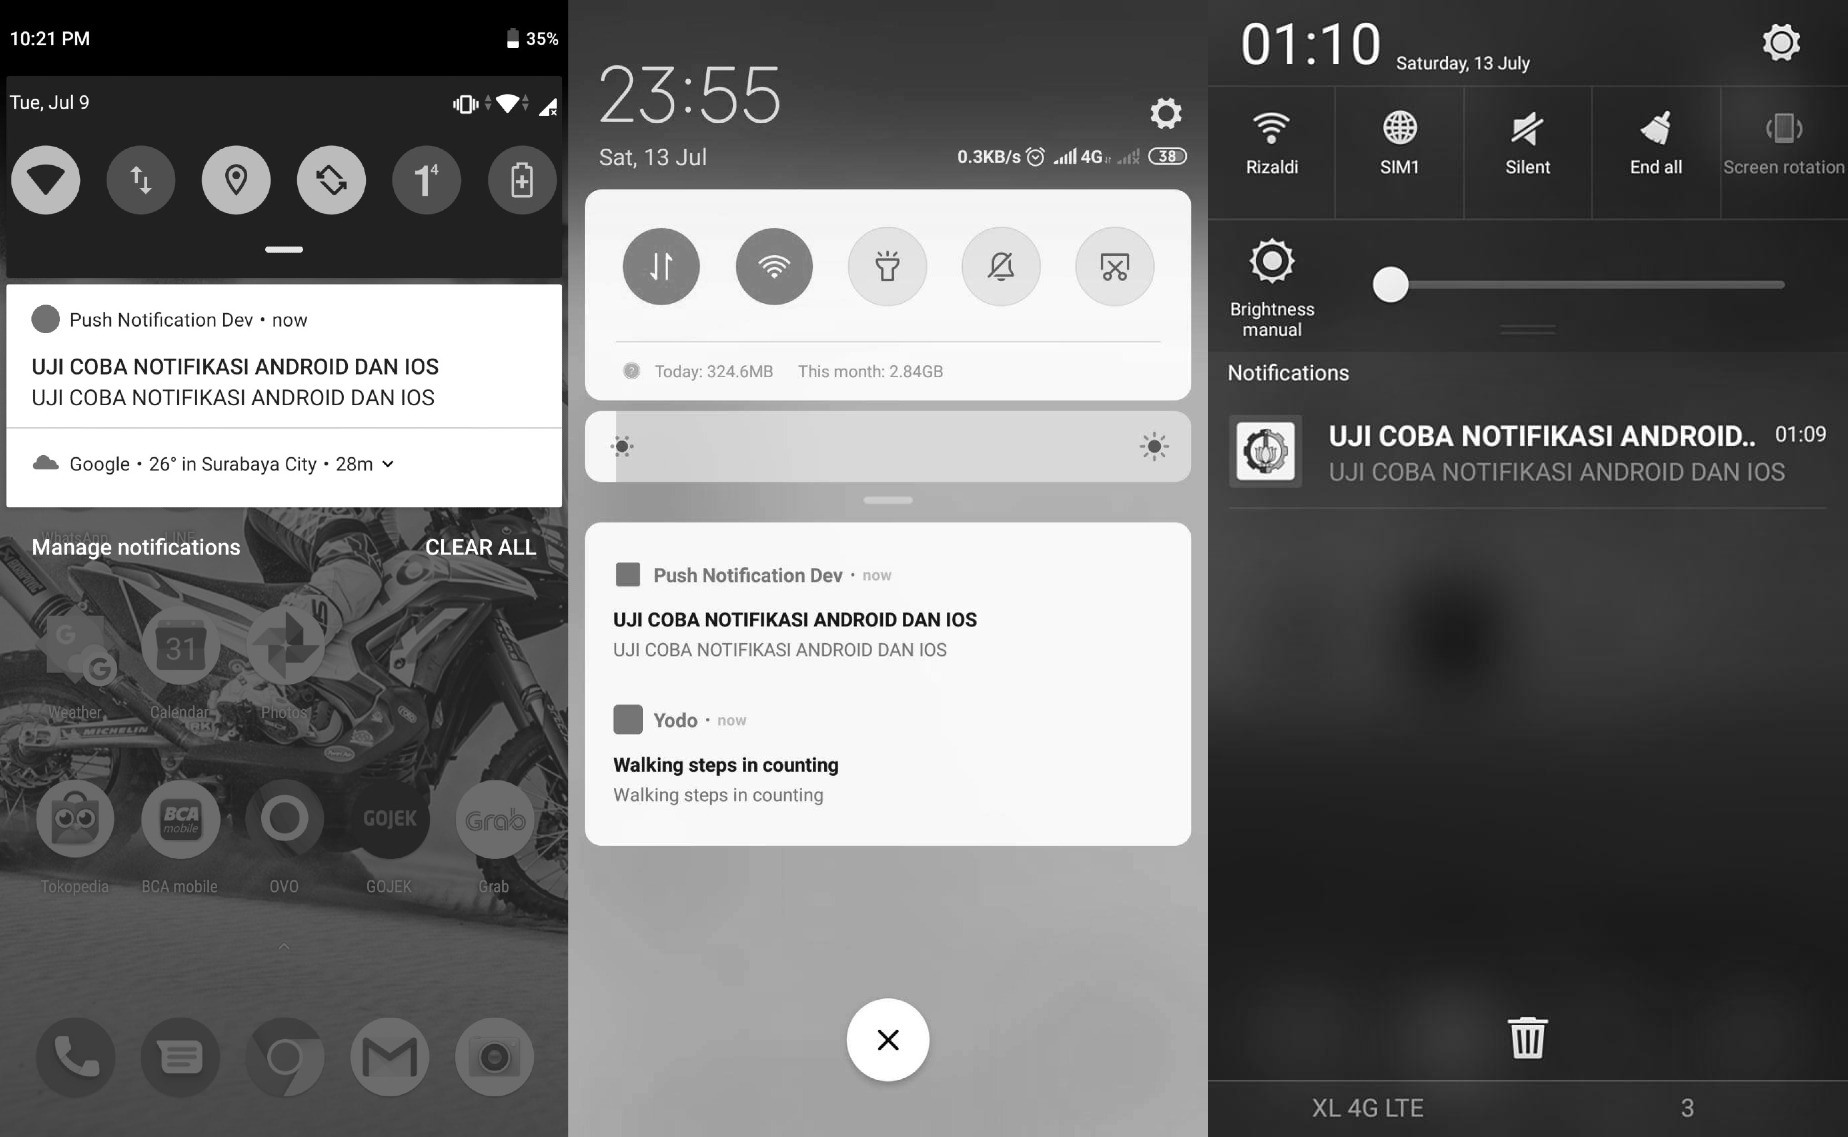
\includegraphics[width=1\textwidth]{bab5/img/notifikasi-android.jpg}
	\caption{Hasil Notifikasi pada Perangkat Android 1, 2, dan 3} \label{img:notifikasi-android}
\end{figure}

\subsection{Pengujian Menampilkan Penggunaan Sumber Daya}
\par Pengujian menampilkan penggunaan sumber daya dilakukan untuk mengetahui apakah Scheduler, Sender APN, dan Sender FCM berhasil menampilkan penggunaan sumber daya dengan tepat. Hasil uji dapat dilihat pada Tabel \ref{t:uji_menampilkan_penggunaan_sumber_daya}.
\begin{longtable}{|>{\columncolor{lightgray}}p{3cm}|p{6.5cm}|}
	\caption{Hasil Uji Menampilkan Penggunaan Sumber Daya} \label{t:uji_menampilkan_penggunaan_sumber_daya} \\ \hline
	\endfirsthead
	Kode & FT-05 \\ \hline
	Nama & Pengujian Menampilkan Penggunaan Sumber Daya \\ \hline
	Tujuan & Menguji apakah sistem mampu menampilkan penggunaan sumber daya \\ \hline
	Kondisi Awal & Scheduler, Sender APN, dan Sender FCM aktif \\ \hline
	Langkah Pengujian &  
	\begin{enumerate}
		\item Pengguna mengakses \textit{endpoint} /actuator/metrics/jvm.memory.used.
		\item Sistem mengembalikan metrik penggunaan memori JVM dalam bentuk JSON.
		\item Pengguna mengakses \textit{endpoint} /actuator/metrics/system.cpu.usage.
		\item Sistem mengembalikan metrik penggunaan CPU dalam bentuk JSON.
	\end{enumerate} \\ \hline
	Hasil yang diharapkan & Aplikasi menampilkan metrik penggunaan Memori dan CPU \\ \hline
	Hasil yang diperoleh & Aplikasi menampilkan metrik penggunaan Memori dan CPU \\ \hline
	Hasil pengujian & Berhasil \\ \hline
\end{longtable}

\subsection{Pengujian Menampilkan Status Kesehatan}
\par Pengujian menampilkan status kesehatan dilakukan untuk mengetahui apakah Scheduler, Sender APN, dan Sender FCM berhasil menampilkan status kesehatan dengan tepat. Hasil uji dapat dilihat pada Tabel \ref{t:uji_menampilkan_status_kesehatan}.
\begin{longtable}{|>{\columncolor{lightgray}}p{3cm}|p{6.5cm}|}
	\caption{Hasil Uji Menampilkan Status Kesehatan} \label{t:uji_menampilkan_status_kesehatan} \\ \hline
	\endfirsthead
	Kode & FT-06 \\ \hline
	Nama & Pengujian Menampilkan Status Kesehatan \\ \hline
	Tujuan & Menguji apakah sistem mampu menampilkan status kesehatan \\ \hline
	Kondisi Awal & Scheduler, Sender APN, dan Sender FCM aktif \\ \hline
	Langkah Pengujian &  
	\begin{enumerate}
		\item Pengguna mengakses \textit{endpoint} /actuator/health.
		\item Sistem mengembalikan metrik kesehatan layanan sistem basis data dan antrian pesan dalam bentuk JSON.
	\end{enumerate} \\ \hline
	Hasil yang diharapkan & Sistem menampilkan status kesehatan sistem basis data dan antrian pesan \\ \hline
	Hasil yang diperoleh & Sistem menampilkan status kesehatan sistem basis data dan antrian pesan \\ \hline
	Hasil pengujian & Berhasil \\ \hline
\end{longtable}

\subsection{Pengujian Menampilkan Konfigurasi}
\par Pengujian menampilkan konfigurasi dilakukan untuk mengetahui apakah Scheduler, Sender APN, dan Sender FCM berhasil menampilkan konfigurasi dengan tepat. Hasil uji dapat dilihat pada Tabel \ref{t:uji_menampilkan_konfigurasi}.
\begin{longtable}{|>{\columncolor{lightgray}}p{3cm}|p{6.5cm}|}
	\caption{Hasil Uji Menampilkan Konfigurasi} \label{t:uji_menampilkan_konfigurasi} \\ \hline
	\endfirsthead
	Kode & FT-07 \\ \hline
	Nama & Pengujian Menampilkan Konfigurasi \\ \hline
	Tujuan & Menguji apakah sistem mampu menampilkan konfigurasi \\ \hline
	Kondisi Awal & Scheduler, Sender APN, dan Sender FCM aktif \\ \hline
	Langkah Pengujian &  
	\begin{enumerate}
		\item Pengguna mengakses \textit{endpoint} /actuator/env.
		\item Sistem mengembalikan konfigurasi sistem dalam bentuk JSON.
	\end{enumerate} \\ \hline
	Hasil yang diharapkan & Sistem menampilkan konfigurasi yang digunakan \\ \hline
	Hasil yang diperoleh & Sistem menampilkan konfigurasi yang digunakan \\ \hline
	Hasil pengujian & Berhasil \\ \hline
\end{longtable}

\subsection{Pengujian Menampilkan Log}
\par Pengujian menampilkan \textit{log} dilakukan untuk mengetahui apakah Scheduler, Sender APN, dan Sender FCM berhasil menampilkan \textit{log} dengan tepat. Hasil uji dapat dilihat pada Tabel \ref{t:uji_menampilkan_log}.
\begin{longtable}{|>{\columncolor{lightgray}}p{3cm}|p{6.5cm}|}
	\caption{Hasil Uji Menampilkan \textit{Log}} \label{t:uji_menampilkan_log} \\ \hline
	\endfirsthead
	Kode & FT-08 \\ \hline
	Nama & Pengujian Menampilkan \textit{Log} \\ \hline
	Tujuan & Menguji apakah sistem mampu menampilkan \textit{log} \\ \hline
	Kondisi Awal & Scheduler, Sender APN, dan Sender FCM aktif \\ \hline
	Langkah Pengujian &  
	\begin{enumerate}
		\item Pengguna mengakses \textit{endpoint} /actuator/logfile.
		\item Sistem mengembalikan isi \textit{log} sistem bentuk teks.
	\end{enumerate} \\ \hline
	Hasil yang diharapkan & Sistem menampilkan isi \textit{log} \\ \hline
	Hasil yang diperoleh & Sistem menampilkan isi \textit{log} \\ \hline
	Hasil pengujian & Berhasil \\ \hline
\end{longtable}

\section{Pengujian Non Fungsional}
\par Pengujian non fungsional dilakukan untuk mengetahui apakah sistem yang dibangun sudah memenuhi standar yang ditentukan, dari aspek performa, keandalan, ketersediaan, dan durabilitas. Skenario pengujian dilakukan dengan mengirim \textit{packet} dengan jumlah besar ke perangkat uji.

\subsection{Pengujian Performa}
\par Pengujian performa dilakukan untuk mengetahui seberapa cepat sistem dalam mengirim \textit{packet} ke layanan APNs dan FCM. Kasus uji dibagi berdasarkan jumlah \textit{packet} yang dikirim secara bersamaan, dengan pengulangan sebanyak 5 kali.
\par Metrik keberhasilan menggunakan durasi waktu pembuatan dan pengiriman \textit{packet}. Durasi pembuatan \textit{packet} dihitung dari waktu \textit{batch} tersimpan di sistem basis data, hingga waktu \textit{batch} selesai diolah. Durasi pengiriman \textit{packet} dihitung dari waktu \textit{batch} dikirim, hingga waktu \textit{packet} terakhir dikirim.

\subsubsection{Pengujian Performa untuk 100 Packet}
\par Skenario pengujian dilakukan dengan membuat \textit{batch} yang menargetkan 50 perangkat iOS dan 50 perangkat Android. Rincian hasil uji dapat dilihat pada Tabel \ref{t:performa-100}.

\begin{longtable}{|p{1.5cm}|p{2cm}|p{2cm}|p{2cm}|}
	\caption{Hasil Uji Performa Pengiriman 100 \textit{Packet}} \label{t:performa-100} \\ \hline
	\rowcolor{lightgray} & \multicolumn{3}{c|}{Durasi Pengolahan \textit{Packet}} \\ \hhline{~|*3{-}|}
	\rowcolor{lightgray} \multirow{-2}{*}{Kode} & Pembuatan & Pengiriman & Total \\ \hline
	\endfirsthead
	\hline
	\rowcolor{lightgray} & \multicolumn{3}{c|}{Durasi Pengolahan \textit{Packet}} \\ \hhline{~|*3{-}|}
	\rowcolor{lightgray} \multirow{-2}{*}{Kode} & Pembuatan & Pengiriman & Total \\ \hline
	\endhead
	NFPT-01 & 0:00:31 & 0:00:52 & 0:01:23 \\ \hline 
	NFPT-02 & 0:00:30 & 0:00:51 & 0:01:21 \\ \hline
	NFPT-03 & 0:00:16 & 0:00:56 & 0:01:11 \\ \hline
	NFPT-04 & 0:00:07 & 0:00:37 & 0:00:44 \\ \hline
	NFPT-05 & 0:00:07 & 0:00:42 & 0:00:48 \\ \hline
\end{longtable}


\subsubsection{Pengujian Performa untuk 500 Packet}
\par Skenario pengujian dilakukan dengan membuat \textit{batch} yang menargetkan 250 perangkat iOS dan 250 perangkat Android. Rincian hasil uji dapat dilihat pada Tabel \ref{t:performa-500}.

\begin{longtable}{|p{1.5cm}|p{2cm}|p{2cm}|p{2cm}|}
	\caption{Hasil Uji Performa Pengiriman 500 \textit{Packet}} \label{t:performa-500} \\ \hline
	\rowcolor{lightgray} & \multicolumn{3}{c|}{Durasi Pengolahan \textit{Packet}} \\ \hhline{~|*3{-}|}
	\rowcolor{lightgray} \multirow{-2}{*}{Kode} & Pembuatan & Pengiriman & Total \\ \hline
	\endfirsthead
	\hline
	\rowcolor{lightgray} & \multicolumn{3}{c|}{Durasi Pengolahan \textit{Packet}} \\ \hhline{~|*3{-}|}
	\rowcolor{lightgray} \multirow{-2}{*}{Kode} & Pembuatan & Pengiriman & Total \\ \hline
	\endhead
	NFPT-06 & 0:00:25 & 0:01:05 & 0:01:29 \\ \hline 
	NFPT-07 & 0:00:43 & 0:00:40 & 0:01:23 \\ \hline
	NFPT-08 & 0:01:50 & 0:00:53 & 0:02:43 \\ \hline
	NFPT-09 & 0:01:02 & 0:01:35 & 0:02:37 \\ \hline
	NFPT-10 & 0:00:31 & 0:01:08 & 0:01:39 \\ \hline
\end{longtable}

\subsubsection{Pengujian Performa untuk 1.000 Packet}
\par Skenario pengujian dilakukan dengan membuat \textit{batch} yang menargetkan 500 perangkat iOS dan 500 perangkat Android. Rincian hasil uji dapat dilihat pada Tabel \ref{t:performa-1k}.

\begin{longtable}{|p{1.5cm}|p{2cm}|p{2cm}|p{2cm}|}
	\caption{Hasil Uji Performa Pengiriman 1.000 \textit{Packet}} \label{t:performa-1k} \\ \hline
	\rowcolor{lightgray} & \multicolumn{3}{c|}{Durasi Pengolahan \textit{Packet}} \\ \hhline{~|*3{-}|}
	\rowcolor{lightgray} \multirow{-2}{*}{Kode} & Pembuatan & Pengiriman & Total \\ \hline
	\endfirsthead
	\hline
	\rowcolor{lightgray} & \multicolumn{3}{c|}{Durasi Pengolahan \textit{Packet}} \\ \hhline{~|*3{-}|}
	\rowcolor{lightgray} \multirow{-2}{*}{Kode} & Pembuatan & Pengiriman & Total \\ \hline
	\endhead
	NFPT-11 & 0:00:21 & 0:02:12 & 0:02:33 \\ \hline 
	NFPT-12 & 0:01:13 & 0:02:02 & 0:03:15 \\ \hline
	NFPT-13 & 0:00:42 & 0:01:55 & 0:02:38 \\ \hline
	NFPT-14 & 0:00:52 & 0:02:06 & 0:02:59 \\ \hline
	NFPT-15 & 0:00:46 & 0:01:57 & 0:02:43 \\ \hline
\end{longtable}

\subsubsection{Pengujian Performa untuk 2.000 Packet}
\par Skenario pengujian dilakukan dengan membuat \textit{batch} yang menargetkan 1.000 perangkat iOS dan 1.000 perangkat Android. Rincian hasil uji dapat dilihat pada Tabel \ref{t:performa-2k}.

\begin{longtable}{|p{1.5cm}|p{2cm}|p{2cm}|p{2cm}|}
	\caption{Hasil Uji Performa Pengiriman 2.000 \textit{Packet}} \label{t:performa-2k} \\ \hline
	\rowcolor{lightgray} & \multicolumn{3}{c|}{Durasi Pengolahan \textit{Packet}} \\ \hhline{~|*3{-}|}
	\rowcolor{lightgray} \multirow{-2}{*}{Kode} & Pembuatan & Pengiriman & Total \\ \hline
	\endfirsthead
	\hline
	\rowcolor{lightgray} & \multicolumn{3}{c|}{Durasi Pengolahan \textit{Packet}} \\ \hhline{~|*3{-}|}
	\rowcolor{lightgray} \multirow{-2}{*}{Kode} & Pembuatan & Pengiriman & Total \\ \hline
	\endhead
	NFPT-16 & 0:00:27 & 0:01:47 & 0:02:14 \\ \hline 
	NFPT-17 & 0:00:15 & 0:01:34 & 0:01:49 \\ \hline
	NFPT-18 & 0:00:28 & 0:01:50 & 0:02:18 \\ \hline
	NFPT-19 & 0:00:05 & 0:02:14 & 0:02:19 \\ \hline
	NFPT-20 & 0:00:25 & 0:01:39 & 0:02:04 \\ \hline
\end{longtable}

\subsubsection{Pengujian Performa untuk 3.000 Packet}
\par Skenario pengujian dilakukan dengan membuat \textit{batch} yang menargetkan 1.500 perangkat iOS dan 1.500 perangkat Android. Rincian hasil uji dapat dilihat pada Tabel \ref{t:performa-3k}.

\begin{longtable}{|p{1.5cm}|p{2cm}|p{2cm}|p{2cm}|}
	\caption{Hasil Uji Performa Pengiriman 3.000 \textit{Packet}} \label{t:performa-3k} \\ \hline
	\rowcolor{lightgray} & \multicolumn{3}{c|}{Durasi Pengolahan \textit{Packet}} \\ \hhline{~|*3{-}|}
	\rowcolor{lightgray} \multirow{-2}{*}{Kode} & Pembuatan & Pengiriman & Total \\ \hline
	\endfirsthead
	\hline
	\rowcolor{lightgray} & \multicolumn{3}{c|}{Durasi Pengolahan \textit{Packet}} \\ \hhline{~|*3{-}|}
	\rowcolor{lightgray} \multirow{-2}{*}{Kode} & Pembuatan & Pengiriman & Total \\ \hline
	\endhead
	NFPT-21 & 0:00:59 & 0:04:05 & 0:05:05 \\ \hline 
	NFPT-22 & 0:01:14 & 0:04:10 & 0:05:24 \\ \hline
	NFPT-23 & 0:01:09 & 0:04:35 & 0:05:44 \\ \hline
	NFPT-24 & 0:00:52 & 0:04:17 & 0:05:09 \\ \hline
	NFPT-25 & 0:00:43 & 0:04:13 & 0:04:56 \\ \hline
\end{longtable}

\subsubsection{Pengujian Performa untuk 20.000 Packet}
\par Skenario pengujian dilakukan dengan membuat \textit{batch} yang menargetkan 10.000 perangkat iOS dan 10.000 perangkat Android. Rincian hasil uji dapat dilihat pada Tabel \ref{t:performa-20k}.
\begin{longtable}{|p{1.5cm}|p{2cm}|p{2cm}|p{2cm}|}
	\caption{Hasil Uji Performa Pengiriman 20.000 \textit{Packet}} \label{t:performa-20k} \\ \hline
	\rowcolor{lightgray} & \multicolumn{3}{c|}{Durasi Pengolahan \textit{Packet}} \\ \hhline{~|*3{-}|}
	\rowcolor{lightgray} \multirow{-2}{*}{Kode} & Pembuatan & Pengiriman & Total \\ \hline
	\endfirsthead
	\hline
	\rowcolor{lightgray} & \multicolumn{3}{c|}{Durasi Pengolahan \textit{Packet}} \\ \hhline{~|*3{-}|}
	\rowcolor{lightgray} \multirow{-2}{*}{Kode} & Pembuatan & Pengiriman & Total \\ \hline
	\endhead
	NFPT-26 & 0:01:42 & 0:15:04 & 0:16:46 \\ \hline 
	NFPT-27 & 0:01:27 & 0:21:34 & 0:23:01 \\ \hline
	NFPT-28 & 0:00:48 & 0:12:10 & 0:12:58 \\ \hline
	NFPT-29 & 0:01:08 & 0:16:17 & 0:17:25 \\ \hline
	NFPT-30 & 0:01:02 & 0:16:17 & 0:17:18 \\ \hline
\end{longtable}

\subsubsection{Pengujian Performa untuk 200.000 Packet}
\par Skenario pengujian dilakukan dengan membuat \textit{batch} yang menargetkan 100.000 perangkat iOS dan 100.000 perangkat Android. Rincian hasil uji dapat dilihat pada Tabel \ref{t:performa-200k}.

\begin{longtable}{|p{1.5cm}|p{2cm}|p{2cm}|p{2cm}|}
\caption{Hasil Uji Performa Pengiriman 200.000 \textit{Packet}} \label{t:performa-200k} \\ \hline
\rowcolor{lightgray} & \multicolumn{3}{c|}{Durasi Pengolahan \textit{Packet}} \\ \hhline{~|*3{-}|}
\rowcolor{lightgray} \multirow{-2}{*}{Kode} & Pembuatan & Pengiriman & Total \\ \hline
\endfirsthead
\hline
\rowcolor{lightgray} & \multicolumn{3}{c|}{Durasi Pengolahan \textit{Packet}} \\ \hhline{~|*3{-}|}
\rowcolor{lightgray} \multirow{-2}{*}{Kode} & Pembuatan & Pengiriman & Total \\ \hline
\endhead
	NFPT-31 & 0:11:00 & 3:06:08 & 3:17:08 \\ \hline 
	NFPT-32 & 0:10:25 & 2:44:55 & 2:55:20 \\ \hline
	NFPT-33 & 0:08:47 & 3:11:12 & 3:20:00 \\ \hline
	NFPT-34 & 0:08:39 & 2:38:49 & 2:47:28 \\ \hline
	NFPT-35 & 0:04:09 & 1:57:47 & 2:01:56 \\ \hline
\end{longtable}

\subsection{Pengujian Keandalan}
\par Pengujian keandalan dilakukan untuk mengetahui tingkat keberhasilan pengiriman \textit{packet} ke perangkat pengguna. Kasus uji dibagi berdasarkan jenis perangkat dan jumlah \textit{packet} yang diuji, dengan pengulangan sebanyak 5 kali.

\subsubsection{Pengujian Keandalan Pengiriman Packet ke Perangkat iOS}
\par Pengujian keandalan pengiriman \textit{packet} ke perangkat iOS dilakukan untuk mengetahui tingkat keberhasilan pengiriman \textit{packet} ke layanan APNs dan perangkat iOS berdasarkan jumlah \textit{packet} yang dikirim secara bersamaan.
\par Metrik keberhasilan menggunakan jumlah \textit{packet} yang diterima oleh Sender APN, APNs dan perangkat iOS, dengan ketentuan sebagai berikut:
\begin{enumerate}
	\item Jumlah \textit{packet} yang diterima oleh Sender APN adalah jumlah \textit{packet} yang berhasil atau gagal.
	\item Jumlah \textit{packet} yang diterima oleh APNs adalah jumlah \textit{packet} yang berhasil atau gagal dengan \textit{error} ApnsClientException.
	\item Jumlah \textit{packet} yang diterima oleh perangkat iOS adalah jumlah \textit{packet} yang berhasil.
\end{enumerate}

\paragraph{Pengujian Keandalan Pengiriman 50 Packet ke Perangkat iOS}
\par Skenario pengujian dilakukan dengan membuat \textit{batch} yang menargetkan 50 pengguna dengan perangkat iOS. Hasil uji dapat diliat pada Tabel \ref{t:keandalan-ios-50}.
\begin{longtable}{|p{1.5cm}|p{2cm}|p{2cm}|p{2cm}|}
	\caption{Hasil Uji Keandalan Pengiriman 50 \textit{Packet} ke Perangkat iOS} \label{t:keandalan-ios-50} \\ \hline
	\rowcolor{lightgray} & \multicolumn{3}{c|}{Jumlah \textit{Packet} Diterima} \\ \hhline{~|*3{-}|}
	\rowcolor{lightgray} \multirow{-2}{*}{Kode} & Sender APN & APNs & iOS \\ \hline
	\endfirsthead
	\hline
	\rowcolor{lightgray} & \multicolumn{3}{c|}{Jumlah \textit{Packet} Diterima} \\ \hhline{~|*3{-}|}
	\rowcolor{lightgray} \multirow{-2}{*}{Kode} & Sender APN & APNs & iOS \\ \hline
	\endhead
	NFAT-01 & 50 & 50 & 50 \\ \hline
	NFAT-02 & 50 & 50 & 50 \\ \hline
	NFAT-03 & 50 & 50 & 50 \\ \hline
	NFAT-04 & 50 & 50 & 50 \\ \hline
	NFAT-05 & 50 & 50 & 50 \\ \hline
\end{longtable}

\paragraph{Pengujian Keandalan Pengiriman 250 Packet ke Perangkat iOS}
\par Skenario pengujian dilakukan dengan membuat \textit{batch} yang menargetkan 250 pengguna dengan perangkat iOS. Hasil uji dapat diliat pada Tabel \ref{t:keandalan-ios-250}.
\begin{longtable}{|p{1.5cm}|p{2cm}|p{2cm}|p{2cm}|}
	\caption{Hasil Uji Keandalan Pengiriman 250 \textit{Packet} ke Perangkat iOS} \label{t:keandalan-ios-250} \\ \hline
	\rowcolor{lightgray} & \multicolumn{3}{c|}{Jumlah \textit{Packet} Diterima} \\ \hhline{~|*3{-}|}
	\rowcolor{lightgray} \multirow{-2}{*}{Kode} & Sender APN & APNs & iOS \\ \hline
	\endfirsthead
	\hline
	\rowcolor{lightgray} & \multicolumn{3}{c|}{Jumlah \textit{Packet} Diterima} \\ \hhline{~|*3{-}|}
	\rowcolor{lightgray} \multirow{-2}{*}{Kode} & Sender APN & APNs & iOS \\ \hline
	\endhead
	NFAT-06 & 250 & 250 & 250 \\ \hline
	NFAT-07 & 250 & 250 & 250 \\ \hline
	NFAT-08 & 250 & 250 & 250 \\ \hline
	NFAT-09 & 250 & 250 & 250 \\ \hline
	NFAT-10 & 250 & 250 & 250 \\ \hline
\end{longtable}

\paragraph{Pengujian Keandalan Pengiriman 500 Packet ke Perangkat iOS}
\par Skenario pengujian dilakukan dengan membuat \textit{batch} yang menargetkan 500 pengguna dengan perangkat iOS. Hasil uji dapat diliat pada Tabel \ref{t:keandalan-ios-500}.
\begin{longtable}{|p{1.5cm}|p{2cm}|p{2cm}|p{2cm}|}
	\caption{Hasil Uji Keandalan Pengiriman 500 \textit{Packet} ke Perangkat iOS} \label{t:keandalan-ios-500} \\ \hline
	\rowcolor{lightgray} & \multicolumn{3}{c|}{Jumlah \textit{Packet} Diterima} \\ \hhline{~|*3{-}|}
	\rowcolor{lightgray} \multirow{-2}{*}{Kode} & Sender APN & APNs & iOS \\ \hline
	\endfirsthead
	\hline
	\rowcolor{lightgray} & \multicolumn{3}{c|}{Jumlah \textit{Packet} Diterima} \\ \hhline{~|*3{-}|}
	\rowcolor{lightgray} \multirow{-2}{*}{Kode} & Sender APN & APNs & iOS \\ \hline
	\endhead
	NFAT-11 & 500 & 500 & 500 \\ \hline
	NFAT-12 & 500 & 500 & 500 \\ \hline
	NFAT-13 & 500 & 500 & 500 \\ \hline
	NFAT-14 & 500 & 500 & 500 \\ \hline
	NFAT-15 & 500 & 500 & 500 \\ \hline
\end{longtable}

\paragraph{Pengujian Keandalan Pengiriman 1.000 Packet ke Perangkat iOS}
\par Skenario pengujian dilakukan dengan membuat \textit{batch} yang menargetkan 1.000 pengguna dengan perangkat iOS. Hasil uji dapat diliat pada Tabel \ref{t:keandalan-ios-1k}.
\begin{longtable}{|p{1.5cm}|p{2cm}|p{2cm}|p{2cm}|}
	\caption{Hasil Uji Keandalan Pengiriman 1.000 \textit{Packet} ke Perangkat iOS} \label{t:keandalan-ios-1k} \\ \hline
	\rowcolor{lightgray} & \multicolumn{3}{c|}{Jumlah \textit{Packet} Diterima} \\ \hhline{~|*3{-}|}
	\rowcolor{lightgray} \multirow{-2}{*}{Kode} & Sender APN & APNs & iOS \\ \hline
	\endfirsthead
	\hline
	\rowcolor{lightgray} & \multicolumn{3}{c|}{Jumlah \textit{Packet} Diterima} \\ \hhline{~|*3{-}|}
	\rowcolor{lightgray} \multirow{-2}{*}{Kode} & Sender APN & APNs & iOS \\ \hline
	\endhead
	NFAT-16 & 1.000 & 1.000 & 1.000 \\ \hline
	NFAT-17 & 1.000 & 1.000 & 1.000 \\ \hline
	NFAT-18 & 1.000 & 1.000 & 1.000 \\ \hline
	NFAT-19 & 1.000 & 1.000 & 1.000 \\ \hline
	NFAT-20 & 1.000 & 1.000 & 1.000 \\ \hline
\end{longtable}

\paragraph{Pengujian Keandalan Pengiriman 1.500 Packet ke Perangkat iOS}
\par Skenario pengujian dilakukan dengan membuat \textit{batch} yang menargetkan 1.500 pengguna dengan perangkat iOS. Hasil uji dapat diliat pada Tabel \ref{t:keandalan-ios-1500}.
\begin{longtable}{|p{1.5cm}|p{2cm}|p{2cm}|p{2cm}|}
	\caption{Hasil Uji Keandalan Pengiriman 1500 \textit{Packet} ke Perangkat iOS} \label{t:keandalan-ios-1500} \\ \hline
	\rowcolor{lightgray} & \multicolumn{3}{c|}{Jumlah \textit{Packet} Diterima} \\ \hhline{~|*3{-}|}
	\rowcolor{lightgray} \multirow{-2}{*}{Kode} & Sender APN & APNs & iOS \\ \hline
	\endfirsthead
	\hline
	\rowcolor{lightgray} & \multicolumn{3}{c|}{Jumlah \textit{Packet} Diterima} \\ \hhline{~|*3{-}|}
	\rowcolor{lightgray} \multirow{-2}{*}{Kode} & Sender APN & APNs & iOS \\ \hline
	\endhead
	NFAT-21 & 1500 & 1500 & 1500 \\ \hline
	NFAT-22 & 1500 & 1500 & 1500 \\ \hline
	NFAT-23 & 1500 & 1500 & 1500 \\ \hline
	NFAT-24 & 1500 & 1500 & 1500 \\ \hline
	NFAT-25 & 1500 & 1500 & 1500 \\ \hline
\end{longtable}

\paragraph{Pengujian Keandalan Pengiriman 10.000 Packet ke Perangkat iOS}
\par Skenario pengujian dilakukan dengan membuat \textit{batch} yang menargetkan 10.000 pengguna dengan perangkat iOS. Hasil uji dan \textit{error} yang terjadi dapat diliat pada Tabel \ref{t:keandalan-ios-10k} dan \ref{t:error-keandalan-ios-10k}.
\begin{longtable}{|p{1.5cm}|p{2cm}|p{2cm}|p{2cm}|}
	\caption{Hasil Uji Keandalan Pengiriman 10.000 \textit{Packet} ke Perangkat iOS} \label{t:keandalan-ios-10k} \\ \hline
	\rowcolor{lightgray} & \multicolumn{3}{c|}{Jumlah \textit{Packet} Diterima} \\ \hhline{~|*3{-}|}
	\rowcolor{lightgray} \multirow{-2}{*}{Kode} & Sender APN & APNs & iOS \\ \hline
	\endfirsthead
	\hline
	\rowcolor{lightgray} & \multicolumn{3}{c|}{Jumlah \textit{Packet} Diterima} \\ \hhline{~|*3{-}|}
	\rowcolor{lightgray} \multirow{-2}{*}{Kode} & Sender APN & APNs & iOS \\ \hline
	\endhead
	NFAT-26 & 10.000 & 10.000 & 9.984 \\ \hline
	NFAT-27 & 10.000 & 10.000 & 9.992 \\ \hline
	NFAT-28 & 10.000 & 10.000 & 9.984 \\ \hline
	NFAT-29 & 10.000 & 10.000 & 9.992 \\ \hline
	NFAT-30 & 10.000 & 10.000 & 9.984 \\ \hline
\end{longtable}
\begin{longtable}{|p{1.5cm}|p{1.5cm}|p{4cm}|}
	\caption{\textit{Error} pada Hasil Uji Keandalan Pengiriman 10.000 \textit{Packet} ke Perangkat iOS} \label{t:error-keandalan-ios-10k} \\ \hline
	\rowcolor{lightgray} Kode & Jumlah & Alasan \\ \hline
	\endfirsthead
	\hline
	\rowcolor{lightgray} Kode & Jumlah & Alasan \\ \hline
	\endhead
	NFAT-26 & 16 & ApnsClientException: TooManyRequests \\ \hline
	NFAT-27 & 8 & ApnsClientException: TooManyRequests \\ \hline
	NFAT-28 & 16 & ApnsClientException: TooManyRequests \\ \hline
	NFAT-29 & 8 & ApnsClientException: TooManyRequests \\ \hline
	NFAT-30 & 16 & ApnsClientException: TooManyRequests \\ \hline
\end{longtable}

\paragraph{Pengujian Keandalan Pengiriman 100.000 Packet ke Perangkat iOS}
\par Skenario pengujian dilakukan dengan membuat \textit{batch} yang menargetkan 100.000 pengguna dengan perangkat iOS. Hasil uji dan \textit{error} yang terjadi dapat diliat pada Tabel \ref{t:keandalan-ios-100k} dan \ref{t:error-keandalan-ios-100k}.
\begin{longtable}{|p{1.5cm}|p{2cm}|p{2cm}|p{2cm}|}
	\caption{Hasil Uji Keandalan Pengiriman 100.000 \textit{Packet} ke Perangkat iOS} \label{t:keandalan-ios-100k} \\ \hline
	\rowcolor{lightgray} & \multicolumn{3}{c|}{Jumlah \textit{Packet} Diterima} \\ \hhline{~|*3{-}|}
	\rowcolor{lightgray} \multirow{-2}{*}{Kode} & Sender APN & APNs & iOS \\ \hline
	\endfirsthead
	\hline
	\rowcolor{lightgray} & \multicolumn{3}{c|}{Jumlah \textit{Packet} Diterima} \\ \hhline{~|*3{-}|}
	\rowcolor{lightgray} \multirow{-2}{*}{Kode} & Sender APN & APNs & iOS \\ \hline
	\endhead
	NFAT-31 & 100.000 & 99.996 & 99.866 \\ \hline
	NFAT-32 & 100.000 & 100.000 & 99.848 \\ \hline
	NFAT-33 & 100.000 & 100.000 & 99.856 \\ \hline
	NFAT-34 & 100.000 & 100.000 & 99.872 \\ \hline
	NFAT-35 & 100.000 & 100.000 & 99.840 \\ \hline
\end{longtable}
\begin{longtable}{|p{1.5cm}|p{1.5cm}|p{4cm}|}
\caption{\textit{Error} pada Hasil Uji Keandalan Pengiriman 100.000 \textit{Packet} ke Perangkat iOS} \label{t:error-keandalan-ios-100k} \\ \hline
\rowcolor{lightgray} Kode & Jumlah & Alasan \\ \hline
 & 130 & ApnsClientException: TooManyRequests \\ \hhline{~|*2{-}|}
\multirow{-1}{*}{NFAT-31} & 4 & IOException: Stream closed before a reply was received \\ \hline
\endfirsthead
\hline
\rowcolor{lightgray} Kode & Jumlah & Alasan \\ \hline
& 130 & ApnsClientException: TooManyRequests \\ \hhline{~|*2{-}|}
\multirow{-1}{*}{NFAT-31} & 4 & IOException: Stream closed before a reply was received \\ \hline
\endhead
NFAT-32 & 152 & ApnsClientException: TooManyRequests \\ \hline
NFAT-33 & 144 & ApnsClientException: TooManyRequests \\ \hline
NFAT-34 & 128 & ApnsClientException: TooManyRequests \\ \hline
NFAT-35 & 160 & ApnsClientException: TooManyRequests \\ \hline
\end{longtable}

\subsubsection{Pengujian Keandalan Pengiriman Packet ke Perangkat Android}
\par Pengujian keandalan pengiriman \textit{packet} ke perangkat Android dilakukan untuk mengetahui tingkat keberhasilan pengiriman \textit{packet} ke layanan FCM dan perangkat Android berdasarkan jumlah \textit{packet} yang dikirim secara bersamaan.
\par Metrik keberhasilan menggunakan jumlah \textit{packet} yang diterima oleh Sender FCM, FCM dan perangkat Android 1, 2, dan 3, dengan ketentuan sebagai berikut:
\begin{enumerate}
	\item Jumlah \textit{packet} yang diterima oleh Sender FCM adalah jumlah \textit{packet} yang berhasil atau gagal.
	\item Jumlah \textit{packet} yang diterima oleh FCM adalah jumlah \textit{packet} yang berhasil atau gagal dengan \textit{error} FirebaseMessagingException.
	\item Jumlah \textit{packet} yang diterima oleh perangkat Android adalah jumlah \textit{packet} yang berhasil.
\end{enumerate}

\paragraph{Pengujian Keandalan Pengiriman 50 Packet ke Perangkat Android}
\par Skenario pengujian dilakukan dengan membuat \textit{batch} yang menargetkan 50 pengguna dengan perangkat Android. Hasil uji dapat diliat pada Tabel \ref{t:keandalan-android-50}.
\begin{longtable}{|p{1.5cm}|p{2cm}|p{1.5cm}|p{1cm}|p{1cm}|p{1cm}|}
	\caption{Hasil Uji Keandalan Pengiriman 50 \textit{Packet} ke Perangkat Android} \label{t:keandalan-android-50} \\ \hline
	\rowcolor{lightgray} & \multicolumn{5}{c|}{Jumlah \textit{Packet} Diterima} \\ \hhline{~|*5{-}|}
	\rowcolor{lightgray} & & & \multicolumn{3}{c|}{Android} \\ \hhline{~~~|*3{-}|}
	\rowcolor{lightgray} \multirow{-3}{*}{Kode} & \multirow{-2}{*}{Sender FCM} & \multirow{-2}{*}{FCM} & 1 & 2 & 3 \\ \hline
	\endfirsthead
	\hline
	\rowcolor{lightgray} & \multicolumn{5}{c|}{Jumlah \textit{Packet} Diterima} \\ \hhline{~|*5{-}|}
	\rowcolor{lightgray} & & & \multicolumn{3}{c|}{Android} \\ \hhline{~~~|*3{-}|}
	\rowcolor{lightgray} \multirow{-3}{*}{Kode} & \multirow{-2}{*}{Sender FCM} & \multirow{-2}{*}{FCM} & 1 & 2 & 3 \\ \hline
	\endhead
	NFAT-36 & 50 & 50 & 16 & 17 & 17 \\ \hline
	NFAT-37 & 50 & 50 & 16 & 17 & 17 \\ \hline
	NFAT-38 & 50 & 50 & 16 & 17 & 17 \\ \hline
	NFAT-39 & 50 & 50 & 16 & 17 & 17 \\ \hline
	NFAT-40 & 50 & 50 & 16 & 17 & 17 \\ \hline
\end{longtable}

\paragraph{Pengujian Keandalan Pengiriman 250 Packet ke Perangkat Android}
\par Skenario pengujian dilakukan dengan membuat \textit{batch} yang menargetkan 250 pengguna dengan perangkat Android. Hasil uji dapat diliat pada Tabel \ref{t:keandalan-android-250}.
\clearpage
\begin{longtable}{|p{1.5cm}|p{2cm}|p{1.5cm}|p{1cm}|p{1cm}|p{1cm}|}
	\caption{Hasil Uji Keandalan Pengiriman 250 \textit{Packet} ke Perangkat Android} \label{t:keandalan-android-250} \\ \hline
	\rowcolor{lightgray} & \multicolumn{5}{c|}{Jumlah \textit{Packet} Diterima} \\ \hhline{~|*5{-}|}
	\rowcolor{lightgray} & & & \multicolumn{3}{c|}{Android} \\ \hhline{~~~|*3{-}|}
	\rowcolor{lightgray} \multirow{-3}{*}{Kode} & \multirow{-2}{*}{Sender FCM} & \multirow{-2}{*}{FCM} & 1 & 2 & 3 \\ \hline
	\endfirsthead
	\hline
	\rowcolor{lightgray} & \multicolumn{5}{c|}{Jumlah \textit{Packet} Diterima} \\ \hhline{~|*5{-}|}
	\rowcolor{lightgray} & & & \multicolumn{3}{c|}{Android} \\ \hhline{~~~|*3{-}|}
	\rowcolor{lightgray} \multirow{-3}{*}{Kode} & \multirow{-2}{*}{Sender FCM} & \multirow{-2}{*}{FCM} & 1 & 2 & 3 \\ \hline
	\endhead
	NFAT-41 & 250 & 250 & 83 & 84 & 83 \\ \hline
	NFAT-42 & 250 & 250 & 83 & 84 & 83 \\ \hline
	NFAT-43 & 250 & 250 & 83 & 84 & 83 \\ \hline
	NFAT-44 & 250 & 250 & 83 & 84 & 83 \\ \hline
	NFAT-45 & 250 & 250 & 83 & 84 & 83 \\ \hline
\end{longtable}

\paragraph{Pengujian Keandalan Pengiriman 500 Packet ke Perangkat Android}
\par Skenario pengujian dilakukan dengan membuat \textit{batch} yang menargetkan 500 pengguna dengan perangkat Android. Hasil uji dapat diliat pada Tabel \ref{t:keandalan-android-500}.
\begin{longtable}{|p{1.5cm}|p{2cm}|p{1.5cm}|p{1cm}|p{1cm}|p{1cm}|}
	\caption{Hasil Uji Keandalan Pengiriman 500 \textit{Packet} ke Perangkat Android} \label{t:keandalan-android-500} \\ \hline
	\rowcolor{lightgray} & \multicolumn{5}{c|}{Jumlah \textit{Packet} Diterima} \\ \hhline{~|*5{-}|}
	\rowcolor{lightgray} & & & \multicolumn{3}{c|}{Android} \\ \hhline{~~~|*3{-}|}
	\rowcolor{lightgray} \multirow{-3}{*}{Kode} & \multirow{-2}{*}{Sender FCM} & \multirow{-2}{*}{FCM} & 1 & 2 & 3 \\ \hline
	\endfirsthead
	\hline
	\rowcolor{lightgray} & \multicolumn{5}{c|}{Jumlah \textit{Packet} Diterima} \\ \hhline{~|*5{-}|}
	\rowcolor{lightgray} & & & \multicolumn{3}{c|}{Android} \\ \hhline{~~~|*3{-}|}
	\rowcolor{lightgray} \multirow{-3}{*}{Kode} & \multirow{-2}{*}{Sender FCM} & \multirow{-2}{*}{FCM} & 1 & 2 & 3 \\ \hline
	\endhead
	NFAT-46 & 500 & 500 & 166 & 167 & 167 \\ \hline
	NFAT-47 & 500 & 500 & 166 & 167 & 167 \\ \hline
	NFAT-48 & 500 & 500 & 166 & 167 & 167 \\ \hline
	NFAT-49 & 500 & 500 & 166 & 167 & 167 \\ \hline
	NFAT-50 & 500 & 500 & 166 & 167 & 167 \\ \hline
\end{longtable}

\paragraph{Pengujian Keandalan Pengiriman 1.000 Packet ke Perangkat Android}
\par Skenario pengujian dilakukan dengan membuat \textit{batch} yang menargetkan 1.000 pengguna dengan perangkat Android. Hasil uji dapat diliat pada Tabel \ref{t:keandalan-android-1k}.
\begin{longtable}{|p{1.5cm}|p{2cm}|p{1.5cm}|p{1cm}|p{1cm}|p{1cm}|}
	\caption{Hasil Uji Keandalan Pengiriman 1.000 \textit{Packet} ke Perangkat Android} \label{t:keandalan-android-1k} \\ \hline
	\rowcolor{lightgray} & \multicolumn{5}{c|}{Jumlah \textit{Packet} Diterima} \\ \hhline{~|*5{-}|}
	\rowcolor{lightgray} & & & \multicolumn{3}{c|}{Android} \\ \hhline{~~~|*3{-}|}
	\rowcolor{lightgray} \multirow{-3}{*}{Kode} & \multirow{-2}{*}{Sender FCM} & \multirow{-2}{*}{FCM} & 1 & 2 & 3 \\ \hline
	\endfirsthead
	\hline
	\rowcolor{lightgray} & \multicolumn{5}{c|}{Jumlah \textit{Packet} Diterima} \\ \hhline{~|*5{-}|}
	\rowcolor{lightgray} & & & \multicolumn{3}{c|}{Android} \\ \hhline{~~~|*3{-}|}
	\rowcolor{lightgray} \multirow{-3}{*}{Kode} & \multirow{-2}{*}{Sender FCM} & \multirow{-2}{*}{FCM} & 1 & 2 & 3 \\ \hline
	\endhead
	NFAT-51 & 1.000 & 1.000 & 333 & 334 & 333 \\ \hline
	NFAT-52 & 1.000 & 1.000 & 333 & 334 & 333 \\ \hline
	NFAT-53 & 1.000 & 1.000 & 333 & 334 & 333 \\ \hline
	NFAT-54 & 1.000 & 1.000 & 333 & 334 & 333 \\ \hline
	NFAT-55 & 1.000 & 1.000 & 333 & 334 & 333 \\ \hline
\end{longtable}

\paragraph{Pengujian Keandalan Pengiriman 1.500 Packet ke Perangkat Android}
\par Skenario pengujian dilakukan dengan membuat \textit{batch} yang menargetkan 1.500 pengguna dengan perangkat Android. Hasil uji dapat diliat pada Tabel \ref{t:keandalan-android-1500}.
\begin{longtable}{|p{1.5cm}|p{2cm}|p{1.5cm}|p{1cm}|p{1cm}|p{1cm}|}
	\caption{Hasil Uji Keandalan Pengiriman 1.500 \textit{Packet} ke Perangkat Android} \label{t:keandalan-android-1500} \\ \hline
	\rowcolor{lightgray} & \multicolumn{5}{c|}{Jumlah \textit{Packet} Diterima} \\ \hhline{~|*5{-}|}
	\rowcolor{lightgray} & & & \multicolumn{3}{c|}{Android} \\ \hhline{~~~|*3{-}|}
	\rowcolor{lightgray} \multirow{-3}{*}{Kode} & \multirow{-2}{*}{Sender FCM} & \multirow{-2}{*}{FCM} & 1 & 2 & 3 \\ \hline
	\endfirsthead
	\hline
	\rowcolor{lightgray} & \multicolumn{5}{c|}{Jumlah \textit{Packet} Diterima} \\ \hhline{~|*5{-}|}
	\rowcolor{lightgray} & & & \multicolumn{3}{c|}{Android} \\ \hhline{~~~|*3{-}|}
	\rowcolor{lightgray} \multirow{-3}{*}{Kode} & \multirow{-2}{*}{Sender FCM} & \multirow{-2}{*}{FCM} & 1 & 2 & 3 \\ \hline
	\endhead
	NFAT-56 & 1.500 & 1.500 & 500 & 500 & 500 \\ \hline
	NFAT-57 & 1.500 & 1.500 & 500 & 500 & 500 \\ \hline
	NFAT-58 & 1.500 & 1.500 & 500 & 500 & 500 \\ \hline
	NFAT-59 & 1.500 & 1.500 & 500 & 500 & 500 \\ \hline
	NFAT-60 & 1.500 & 1.500 & 500 & 500 & 500 \\ \hline
\end{longtable}

\paragraph{Pengujian Keandalan Pengiriman 10.000 Packet ke Perangkat Android}
\par Skenario pengujian dilakukan dengan membuat \textit{batch} yang menargetkan 10.000 pengguna dengan perangkat Android. Hasil uji dapat diliat pada Tabel \ref{t:keandalan-android-10k}.
\begin{longtable}{|p{1.5cm}|p{2cm}|p{1.5cm}|p{1cm}|p{1cm}|p{1cm}|}
	\caption{Hasil Uji Keandalan Pengiriman 10.000 \textit{Packet} ke Perangkat Android} \label{t:keandalan-android-10k} \\ \hline
	\rowcolor{lightgray} & \multicolumn{5}{c|}{Jumlah \textit{Packet} Diterima} \\ \hhline{~|*5{-}|}
	\rowcolor{lightgray} & & & \multicolumn{3}{c|}{Android} \\ \hhline{~~~|*3{-}|}
	\rowcolor{lightgray} \multirow{-3}{*}{Kode} & \multirow{-2}{*}{Sender FCM} & \multirow{-2}{*}{FCM} & 1 & 2 & 3 \\ \hline
	\endfirsthead
	\hline
	\rowcolor{lightgray} & \multicolumn{5}{c|}{Jumlah \textit{Packet} Diterima} \\ \hhline{~|*5{-}|}
	\rowcolor{lightgray} & & & \multicolumn{3}{c|}{Android} \\ \hhline{~~~|*3{-}|}
	\rowcolor{lightgray} \multirow{-3}{*}{Kode} & \multirow{-2}{*}{Sender FCM} & \multirow{-2}{*}{FCM} & 1 & 2 & 3 \\ \hline
	\endhead
	NFAT-61 & 10.000 & 10.000 & 3.333 & 3.334 & 3.333 \\ \hline
	NFAT-62 & 10.000 & 10.000 & 3.333 & 3.334 & 3.333 \\ \hline
	NFAT-63 & 10.000 & 10.000 & 3.333 & 3.334 & 3.333 \\ \hline
	NFAT-64 & 10.000 & 10.000 & 3.333 & 3.334 & 3.333 \\ \hline
	NFAT-65 & 10.000 & 10.000 & 3.333 & 3.334 & 3.333 \\ \hline
\end{longtable}

\paragraph{Pengujian Keandalan Pengiriman 100.000 Packet ke Perangkat Android}
\par Skenario pengujian dilakukan dengan membuat \textit{batch} yang menargetkan 100.000 pengguna dengan perangkat Android. Hasil uji dan \textit{error} yang terjadi dapat diliat pada Tabel \ref{t:keandalan-android-100k} dan \ref{t:error-keandalan-android-100k}.
\begin{longtable}{|p{1.5cm}|p{2cm}|p{1.5cm}|p{1cm}|p{1cm}|p{1cm}|}
	\caption{Hasil Uji Keandalan Pengiriman 100.000 \textit{Packet} ke Perangkat Android} \label{t:keandalan-android-100k} \\ \hline
	\rowcolor{lightgray} & \multicolumn{5}{c|}{Jumlah \textit{Packet} Diterima} \\ \hhline{~|*5{-}|}
	\rowcolor{lightgray} & & & \multicolumn{3}{c|}{Android} \\ \hhline{~~~|*3{-}|}
	\rowcolor{lightgray} \multirow{-3}{*}{Kode} & \multirow{-2}{*}{Sender FCM} & \multirow{-2}{*}{FCM} & 1 & 2 & 3 \\ \hline
	\endfirsthead
	\hline
	\rowcolor{lightgray} & \multicolumn{5}{c|}{Jumlah \textit{Packet} Diterima} \\ \hhline{~|*5{-}|}
	\rowcolor{lightgray} & & & \multicolumn{3}{c|}{Android} \\ \hhline{~~~|*3{-}|}
	\rowcolor{lightgray} \multirow{-3}{*}{Kode} & \multirow{-2}{*}{Sender FCM} & \multirow{-2}{*}{FCM} & 1 & 2 & 3 \\ \hline
	\endhead
	NFAT-66 & 100.000 & 100.000 & 33.333 & 33.334 & 33.333 \\ \hline
	NFAT-67 & 100.000 & 100.000 & 33.333 & 33.334 & 33.333 \\ \hline
	NFAT-68 & 100.000 & 100.000 & 33.333 & 33.334 & 33.333 \\ \hline
	NFAT-69 & 100.000 & 100.000 & 33.333 & 33.333 & 33.333 \\ \hline
	NFAT-70 & 100.000 & 100.000 & 33.333 & 33.334 & 33.333 \\ \hline
\end{longtable}

\begin{longtable}{|p{1.5cm}|p{1.5cm}|p{5cm}|}
	\caption{\textit{Error} pada Hasil Uji Keandalan Pengiriman 100.000 \textit{Packet} ke Perangkat Android} \label{t:error-keandalan-android-100k} \\ \hline
	\rowcolor{lightgray} Kode & Jumlah & Alasan \\ \hline
	\endfirsthead
	\hline
	\rowcolor{lightgray} Kode & Jumlah & Alasan \\ \hline
	\endhead
	NFAT-69 & 1 & FirebaseMessagingException: The service is currently unavailable. \\ \hline
\end{longtable}

\subsection{Pengujian Ketersediaan}
\par Pengujian ketersediaan dilakukan untuk mengetahui apakah sistem tetap bekerja normal saat sedang mengirimkan \textit{packet} dalam jumlah besar.
\par Metrik keberhasilan menggunakan jumlah server mengalami \textit{down} (berhenti beroperasi). Pengecekan kondisi \textit{down} dilakukan dengan mengecek status kesehatan lewat API Actuator setiap 15 menit.

\subsubsection{Pengujian Ketersediaan untuk Pengiriman 2.000 Packet}
\par Skenario pengujian dilakukan dengan membuat \textit{batch} yang menargetkan 1.000 perangkat iOS dan 1.000 perangkat Android. Rincian hasil uji dapat dilihat pada Tabel \ref{t:ketersediaan-2k}.
\begin{longtable}{|p{1.5cm}|p{2cm}|p{2cm}|p{2cm}|}
	\caption{Hasil Uji Ketersediaan Layanan untuk Pengiriman 2.000 \textit{Packet}} \label{t:ketersediaan-2k} \\ \hline
	\rowcolor{lightgray} & \multicolumn{3}{c|}{Jumlah \textit{Down}} \\ \hhline{~|*3{-}|}
	\rowcolor{lightgray} \multirow{-2}{*}{Kode}  & Scheduler & Sender APN & Sender FCM \\ \hline
	\endfirsthead
	\hline
	\rowcolor{lightgray} & \multicolumn{3}{c|}{Jumlah \textit{Down}} \\ \hhline{~|*3{-}|}
	\rowcolor{lightgray} \multirow{-2}{*}{Kode}  & Scheduler & Sender APN & Sender FCM \\ \hline
	\endhead
	NFTT-01 & 0 & 0 & 0 \\ \hline
	NFTT-02 & 0 & 0 & 0 \\ \hline
	NFTT-03 & 0 & 0 & 0 \\ \hline
	NFTT-04 & 0 & 0 & 0 \\ \hline
	NFTT-05 & 0 & 0 & 0 \\ \hline
\end{longtable}

\subsubsection{Pengujian Ketersediaan untuk Pengiriman 20.000 Packet}
\par Skenario pengujian dilakukan dengan membuat \textit{batch} yang menargetkan 10.000 perangkat iOS dan 10.000 perangkat Android. Rincian hasil uji dapat dilihat pada Tabel \ref{t:ketersediaan-20k}.
\begin{longtable}{|p{1.5cm}|p{2cm}|p{2cm}|p{2cm}|}
	\caption{Hasil Uji Ketersediaan Layanan untuk Pengiriman 20.000 \textit{Packet}} \label{t:ketersediaan-20k} \\ \hline
	\rowcolor{lightgray} & \multicolumn{3}{c|}{Jumlah \textit{Down}} \\ \hhline{~|*3{-}|}
	\rowcolor{lightgray} \multirow{-2}{*}{Kode}  & Scheduler & Sender APN & Sender FCM \\ \hline
	\endfirsthead
	\hline
	\rowcolor{lightgray} & \multicolumn{3}{c|}{Jumlah \textit{Down}} \\ \hhline{~|*3{-}|}
	\rowcolor{lightgray} \multirow{-2}{*}{Kode}  & Scheduler & Sender APN & Sender FCM \\ \hline
	\endhead
	NFTT-06 & 0 & 0 & 0 \\ \hline
	NFTT-07 & 0 & 0 & 0 \\ \hline
	NFTT-08 & 0 & 0 & 0 \\ \hline
	NFTT-09 & 0 & 0 & 0 \\ \hline
	NFTT-10 & 0 & 0 & 0 \\ \hline
\end{longtable}

\subsubsection{Pengujian Ketersediaan untuk Pengiriman 200.000 Packet}
\par Skenario pengujian dilakukan dengan membuat \textit{batch} yang menargetkan 100.000 perangkat iOS dan 100.000 perangkat Android. Rincian hasil uji dapat dilihat pada Tabel \ref{t:ketersediaan-200k}.
\begin{longtable}{|p{1.5cm}|p{2cm}|p{2cm}|p{2cm}|}
	\caption{Hasil Uji Ketersediaan Layanan untuk Pengiriman 200.000 \textit{Packet}} \label{t:ketersediaan-200k} \\ \hline
	\rowcolor{lightgray} & \multicolumn{3}{c|}{Jumlah \textit{Down}} \\ \hhline{~|*3{-}|}
	\rowcolor{lightgray} \multirow{-2}{*}{Kode}  & Scheduler & Sender APN & Sender FCM \\ \hline
	\endfirsthead
	\hline
	\rowcolor{lightgray} & \multicolumn{3}{c|}{Jumlah \textit{Down}} \\ \hhline{~|*3{-}|}
	\rowcolor{lightgray} \multirow{-2}{*}{Kode}  & Scheduler & Sender APN & Sender FCM \\ \hline
	\endhead
	NFTT-11 & 0 & 0 & 0 \\ \hline
	NFTT-12 & 0 & 0 & 0 \\ \hline
	NFTT-13 & 0 & 0 & 0 \\ \hline
	NFTT-14 & 0 & 0 & 0 \\ \hline
	NFTT-15 & 0 & 0 & 0 \\ \hline
\end{longtable}

\subsection{Pengujian Durabilitas}
\par Pengujian durabilitas dilakukan untuk mengetahui apakah pesan yang sudah berada di sistem antrian pesan tetap dapat terkirim jika salah satu komponen aplikasi mati sementara. Pengujian dibagi menjadi 3 skenario, yaitu saat Kafka dimatikan, Sender APN dimatikan dan Sender FCM dimatikan.

\subsubsection{Pengujian Mematikan Sementara Kafka}
\par Pengujian mematikan sementara Kafka dilakukan dengan cara mematikan Kafka selama 5 menit ditengah proses pengiriman \textit{packet}. Hasil uji dapat dilihat pada Tabel \ref{t:nft_kafka_mati}.
\begin{longtable}{|>{\columncolor{lightgray}}p{3cm}|p{6.5cm}|}
	\caption{Hasil Uji Mematikan Sementara Kafka} \label{t:nft_kafka_mati} \\ \hline
	\endfirsthead
	Kode & NFDT-01 \\ \hline
	Nama & Pengujian Mematikan Sementara Kafka \\ \hline
	Tujuan & Mengetahui apakah sistem mampu mengirimkan \textit{push notification} jika Sender FCM mati sementara \\ \hline
	Kondisi Awal & Sistem dalam keadaan berjalan \\ \hline
	Langkah Pengujian &  
	\begin{enumerate}
		\item Aktor membuat \textit{batch} baru lewat halaman kirim notifikasi pada modul manajemen.
		\item Kafka menerima \textit{packet} dari \textit{batch}
		\item Kafka dimatikan selama 5 menit.
	\end{enumerate} \\ \hline
	Hasil yang diharapkan & Notifikasi diterima oleh perangkat Android \\ \hline
	Hasil yang diperoleh & Notifikasi diterima oleh perangkat Android \\ \hline
	Hasil pengujian & Berhasil \\ \hline
\end{longtable}

\subsubsection{Pengujian Mematikan Sementara Sender APN}
\par Pengujian mematikan sementara Sender APN dilakukan dengan cara mematikan Sender APN selama 5 menit ditengah proses pengiriman \textit{packet}. Hasil uji dapat dilihat pada Tabel \ref{t:nft_sender_apn_mati}.
\begin{longtable}{|>{\columncolor{lightgray}}p{3cm}|p{6.5cm}|}
	\caption{Hasil Uji Mematikan Sementara Sender APN} \label{t:nft_sender_apn_mati} \\ \hline
	\endfirsthead
	Kode & NFDT-02 \\ \hline
	Nama & Pengujian Mematikan Sementara Sender APN \\ \hline
	Tujuan & Mengetahui apakah sistem mampu mengirimkan \textit{push notification} jika Sender APN mati sementara \\ \hline
	Kondisi Awal & Sistem dalam keadaan berjalan \\ \hline
	Langkah Pengujian &  
	\begin{enumerate}
		\item Aktor membuat \textit{batch} baru lewat halaman kirim notifikasi pada modul manajemen.
		\item Kafka menerima \textit{packet} dari \textit{batch}
		\item Sender APN dimatikan selama 5 menit.
	\end{enumerate} \\ \hline
	Hasil yang diharapkan & Notifikasi diterima oleh perangkat iOS \\ \hline
	Hasil yang diperoleh & Notifikasi diterima oleh perangkat iOS \\ \hline
	Hasil pengujian & Berhasil \\ \hline
\end{longtable}

\subsubsection{Pengujian Mematikan Sementara Sender FCM}
\par Pengujian mematikan sementara Sender FCM dilakukan dengan cara mematikan Sender FCM selama 5 menit ditengah proses pengiriman \textit{packet}. Hasil uji dapat dilihat pada Tabel \ref{t:nft_sender_fcm_mati}.
\begin{longtable}{|>{\columncolor{lightgray}}p{3cm}|p{6.5cm}|}
	\caption{Hasil Uji Mematikan Sementara Sender FCM} \label{t:nft_sender_fcm_mati} \\ \hline
	\endfirsthead
	Kode & NFDT-03 \\ \hline
	Nama & Pengujian Mematikan Sementara Sender FCM \\ \hline
	Tujuan & Mengetahui apakah sistem mampu mengirimkan \textit{push notification} jika Sender FCM mati sementara \\ \hline
	Kondisi Awal & Sistem dalam keadaan berjalan \\ \hline
	Langkah Pengujian &  
	\begin{enumerate}
		\item Aktor membuat \textit{batch} baru lewat halaman kirim notifikasi pada modul manajemen.
		\item Kafka menerima \textit{packet} dari \textit{batch}
		\item Sender FCM dimatikan selama 5 menit.
	\end{enumerate} \\ \hline
	Hasil yang diharapkan & Notifikasi diterima oleh perangkat Android \\ \hline
	Hasil yang diperoleh & Notifikasi diterima oleh perangkat Android \\ \hline
	Hasil pengujian & Berhasil \\ \hline
\end{longtable}

\section{Evaluasi Hasil Pengujian}
\par Evaluasi hasil pengujian membahas apakah kebutuhan fungsional dan non fungsional aplikasi sudah terpenuhi berdasarkan hasil pengujian yang dilakukan, penyebab kegagalan pada saat pengujian, serta perbandingan dengan aplikasi sebelumnya.

\subsection{Evaluasi Hasil Pengujian Fungsional}
\par Berdasarkan hasil uji, dapat dikatakan bahwa aplikasi Push Notification Terpusat yang dibangun pada tugas akhir ini sudah memenuhi semua fungsionalitas dibutuhkan. Rangkuman kebutuhan fungsional serta pengujian yang dilakukan dapat dilihat pada Tabel \ref{t:eval_f}.
\begin{longtable}{|p{1.5cm}|p{3.5cm}|p{1.5cm}|p{1.5cm}|}
	\caption{Rangkuman Hasil Uji Fungsional} \label{t:eval_f} \\ \hline
	\rowcolor{lightgray} Kode Kebutuhan & Nama Kebutuhan & Kode Uji & Hasil \\ \hline
	\endfirsthead
	\hline
	\rowcolor{lightgray} Kode Kebutuhan & Nama Kebutuhan & Kode Uji & Hasil \\ \hline
	\endhead
	F-01 & Pembuatan \textit{Packet} & FT-01 & Berhasil \\ \hline
	F-02 & Menambahkan \textit{Packet} ke Antrian & FT-02 & Berhasil \\ \hline
	F-03 & Pengiriman \textit{Packet} ke APNs & FT-03 & Berhasil \\ \hline
	F-04 & Pengiriman \textit{Packet} ke FCM & FT-04 & Berhasil \\ \hline
	F-05 & Menampilkan Penggunaan Sumber Daya & FT-05 & Berhasil \\ \hline
	F-06 & Menampilkan Status Kesehatan & FT-06 & Berhasil \\ \hline
	F-07 & Menampilkan Konfigurasi & FT-07 & Berhasil \\ \hline
	F-08 & Menampilkan \textit{Log} & FT-08 & Berhasil \\ \hline
\end{longtable}

\subsection{Evaluasi Perbandingan Hasil Pengujian Performa}
\par Evaluasi hasil pengujian performa dilakukan dengan membandingkan hasil uji pada penelitian sebelumnya dengan yang didapatkan pada tugas akhir ini. Pada penelitian sebelumnya, performa diukur dengan menghitung rata-rata waktu yang dibutuhkan untuk mengirim satu \textit{request} ke layanan APNs dan FCM. Sebagai pembanding yang sepadan, rata-rata per-\textit{request} pada penelitian sebelumnya akan dikalikan dengan jumlah notifikasi yang dikirim dan dibandingkan dengan total waktu pengolahan \textit{packet} pada tugas akhir ini.
\par Berdasarkan hasil uji, untuk kasus uji kurang dari 100 notifikasi, aplikasi yang dibangun berjalan hingga 2 kali lebih lambat. Namun, untuk kasus uji lebih dari 500 notifikasi, aplikasi yang dibangun pada tugas akhir ini mampu mengirim hingga 138 kali lebih cepat.
\par Untuk kasus uji dibawah 100 notifikasi, pengiriman berjalan lebih lambat karena notifikasi dibuat dan dikirim oleh Scheduler setiap 30 detik. Sementara itu, untuk kasus uji diatas 500, peningkatan kecepatan pengiriman disebabkan oleh arsitektur antrian pesan yang digunakan oleh Kafka, yang memungkinkan pemrosesan data secara bersamaan dengan membagi antrian berdasarkan topik dan partisi.
\par Rincian perbandingan hasil uji performa dengan penelitian sebelumnya dapat dilihat pada Tabel \ref{t:perbandingan-performa}.
\begin{longtable}{|p{0.5cm}|p{3cm}|p{2.5cm}|p{2.5cm}|}
	\caption{Perbandingan Hasil Uji Performa} \label{t:perbandingan-performa} \\ \hline
	\rowcolor{lightgray} & & \multicolumn{2}{c|}{Rata-Rata Total} \\ \hhline{~~|*2{-}|}
	\rowcolor{lightgray} \multirow{-2}{*}{No} & \multirow{-2}{*}{Jumlah Notifikasi} & Lama & Baru \\ \hline
	\endfirsthead
	\hline
	\rowcolor{lightgray} & & \multicolumn{2}{c|}{Rata-Rata Total} \\ \hhline{~~|*2{-}|}
	\rowcolor{lightgray} \multirow{-2}{*}{No} & \multirow{-2}{*}{Jumlah Notifikasi} & Lama & Baru \\ \hline
	\endhead
	1 & 100 & 0:00:33 & 0:01:06 \\ \hline
	2 & 500 & 0:19:23 & 0:01:58 \\ \hline
	3 & 1.000 & 1:17:44 & 0:02:50 \\ \hline
	4 & 2.000 & 4:56:18 & 0:02:09 \\ \hline
	5 & 3.000 & 8:47:36 & 0:05:16 \\ \hline
	6 & 20.000 & - & 0:17:30 \\ \hline
	7 & 200.000 & - & 2:52:22 \\ \hline
\end{longtable}

\subsection{Evaluasi Perbandingan Hasil Pengujian Keandalan}
\par Evaluasi hasil pengujian keandalan dilakukan dengan membandingkan hasil uji pada penelitian sebelumnya dengan yang didapatkan pada tugas akhir ini. Pada penelitian sebelumnya, keandalan diukur dengan menghitung seberapa banyak \textit{request} yang berhasil dikirimkan ke layanan APNs dan FCM. Sebagai pembanding yang sepadan, keandalan pada tugas akhir ini akan diukur dengan menghitung seberapa banyak \textit{packet} yang diterima oleh layanan APNs dan FCM.
\par Berdasarkan hasil uji, dapat dikatakan bahwa tingkat keberhasilan pengiriman notifikasi menjadi jauh lebih baik dari sebelumnya. Aplikasi pada penelitian sebelumnya hanya mampu mengirim rata-rata 63,8 persen dari 3.000 notifikasi yang dikirim, yang berarti aplikasi hanya mampu mengirim hingga 1.900 notifikasi dalam satu waktu. Aplikasi pada tugas akhir ini berhasil mengirim 200.000 notifikasi dengan rata-rata tingkat keberhasilan 99,99 persen, yang berarti aplikasi mampu mengirim hingga 199.980 notifikasi dalam satu waktu.
\par Peningkatan tingkat keberhasilan pengiriman notifikasi ini disebabkan oleh arsitektur antrian pesan yang digunakan oleh Kafka, yang menjamin bahwa hanya ada 1 \textit{consumer} yang dapat menggunakan antrian yang ada pada topik dan antrian yang sama, sehingga tidak ada \textit{consumer} yang berebut untuk mengambil pesan.
\par Rincian perbandingan hasil uji keandalan dengan penelitian sebelumnya dapat dilihat pada Tabel \ref{t:perbandingan-keandalan}.
\begin{longtable}{|p{0.5cm}|p{3cm}|p{2.5cm}|p{2.5cm}|}
	\caption{Perbandingan Hasil Uji Keandalan} \label{t:perbandingan-keandalan} \\ \hline
	\rowcolor{lightgray} & & \multicolumn{2}{c|}{Rata-Rata Tingkat Keberhasilan} \\ \hhline{~~|*2{-}|}
	\rowcolor{lightgray} \multirow{-2}{*}{No} & \multirow{-2}{*}{Jumlah Notifikasi} & Lama & Baru \\ \hline
	\endfirsthead
	\hline
	\rowcolor{lightgray} & & \multicolumn{2}{c|}{Rata-Rata Tingkat Keberhasilan} \\ \hhline{~~|*2{-}|}
	\rowcolor{lightgray} \multirow{-2}{*}{No} & \multirow{-2}{*}{Jumlah Notifikasi} & Lama & Baru \\ \hline
	\endhead
	1 & 100 & 100\% & 100\% \\ \hline
	2 & 500 & 100\% & 100\% \\ \hline
	3 & 1000 & 100\% & 100\% \\ \hline
	4 & 2.000 & 80,7\% & 100\% \\ \hline
	5 & 3.000 & 63,8\% & 100\% \\ \hline
	6 & 20.000 & - & 100\% \\ \hline
	7 & 200.000 & - & 99,99\% \\ \hline
\end{longtable}

\subsection{Evaluasi Kegagalan pada Hasil Pengujian Keandalan}
\par Pada pengujian keandalan, sebagian besar notifikasi gagal dikirim karena permintaan notifikasi ditolak oleh layanan APNs dan FCM karena dianggap \textit{spam} akibat terlalu banyak mengirim notifikasi ke satu perangkat. Selain itu, koneksi internet yang lambat atau terputus juga menjadi penyebab sebagian notifikasi gagal dikirim. Rincian \textit{error} dan penyebabnya dapat dilihat pada Tabel \ref{t:penyebab-gagal}.
\begin{longtable}{|p{0.5cm}|p{4.5cm}|p{4cm}|}
	\caption{Penyebab Kegagalan pada Hasil Uji Keandalan} \label{t:penyebab-gagal} \\ \hline
	\rowcolor{lightgray} No & \textit{Error} & Penyebab \\ \hline
	\endfirsthead
	\hline
	\rowcolor{lightgray} No & \textit{Error} & Penyebab \\ \hline
	\endhead
	1 & ApnsClientException: TooManyRequests & APNs memblokir \textit{request} karena dianggap spam. \\ \hline
	2 & IOException: Stream closed before a reply was received & Gagal menerima \textit{response}, disebabkan oleh koneksi lambat atau terputus. \\ \hline
	3 & FirebaseMessagingException: The service is currently unavailable & FCM memblokir \textit{request} karena dianggap spam. \\ \hline
\end{longtable}

\subsection{Evaluasi Hasil Pengujian Ketersediaan}
\par Evaluasi hasil pengujian ketersediaan dilakukan dengan menghitung jumlah server mengalami \textit{down} ketika sedang mengirim notifikasi dalam jumlah besar. Berdasarkan hasil uji, sistem tidak mengalami \textit{down} sama sekali saat digunakan untuk mengirim hingga 200.000 notifikasi.
\par Tidak adanya \textit{down} ini disebabkan oleh penggunaan antrian pesan dalam pengiriman notifikasi. Dengan penggunaan antrian pesan, sistem hanya akan mengolah tugas yang mampu untuk dikerjakan, sehingga beban komputasi tidak akan melebihi kapasitas server. Rangkuman hasil uji ketersediaan dapat dilihat pada Tabel \ref{t:rangkuman-ketersediaan}.
\begin{longtable}{|p{0.5cm}|p{3cm}|p{4cm}|}
	\caption{Rangkuman Hasil Uji Ketersediaan} \label{t:rangkuman-ketersediaan} \\ \hline
	\rowcolor{lightgray} No & Jumlah Notifikasi & Rata-Rata Jumlah \textit{Down} \\ \hline
	\endfirsthead
	\hline
	\rowcolor{lightgray} No & Jumlah Notifikasi & Rata-Rata Jumlah \textit{Down} \\ \hline
	\endhead
	1 & 2.000 & 0 \\ \hline
	2 & 20.000 & 0 \\ \hline
	3 & 200.000 & 0 \\ \hline
\end{longtable}

\subsection{Evaluasi Hasil Pengujian Durabilitas}
\par Evaluasi hasil pengujian durabilitas dilakukan dengan menghitung berapa banyak pesan yang tidak terkirim saat salah satu komponen yang ada di sistem dimatikan sementara.
\par Berdasarkan hasil uji, \textit{packet} yang sudah disimpan di Kafka tetap berhasil terkirim meskipun Kafka, Sender APN, atau Sender FCM dimatikan saat proses pengiriman \textit{packet} sedang berlangsung. Rangkuman hasil uji dapat dilihat pada Tabel \ref{t:rangkuman-durabilitas}.
\begin{longtable}{|p{0.5cm}|p{3.5cm}|p{2cm}|}
	\caption{Rangkuman Hasil Uji Durabilitas} \label{t:rangkuman-durabilitas} \\ \hline
	\rowcolor{lightgray} No & Komponen Dimatikan & Hasil \\ \hline 
	\endfirsthead
	\hline
	\rowcolor{lightgray} No & Komponen Dimatikan & Hasil \\ \hline 
	\endhead
	1 & Kafka & Berhasil \\ \hline
	2 & Sender APN & Berhasil \\ \hline
	3 & Sender FCM & Berhasil \\ \hline
\end{longtable}
